\section{微波网络理论}

任何一个微波系统都是由各种微波元件和微波传输线组成的。微波传输线的特性可以用广义传输线方程来描述,微波元件的特性可以用类似于低频网络的等效电路来描述。因此,任何一个复杂的微波系统都可以用电磁场理论和低频网络理论相结合的方法来分析,这种理论称为微波网络理论。

\subsection{二端口微波网络的网络参量}

在各种微波网络中,二端口微波网络是最基本的。例如,衰减器、移相器、阻抗变换器和滤波器等均属于二端口微波网络。对于一个线性二端口微波网络,应用叠加定理,可以得到表征网络特性的线性方程组。

表征二端口微波网络的参数可以分为两大类:一类是反映网络参考面上电压与电流之间关系的参数,对于图 4-4-1 中的二端口微波网络,参考面 T 1​和 T 2​上的电压和电流方向如图 4-4-1(a) 所示。另一类是反映网络参考面上入射波电压与反射波电压之间关系的参数,如图 4-4-1(b) 所示。

\begin{figure}
	\centering
	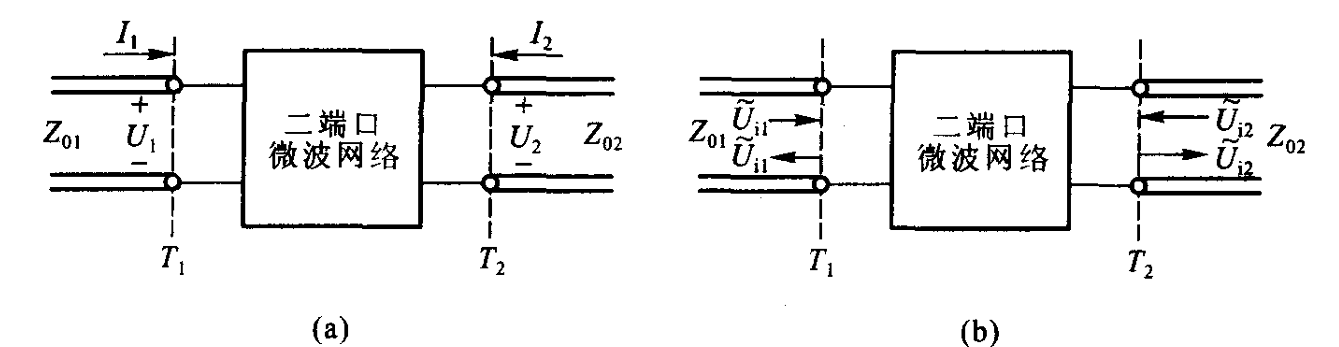
\includegraphics[width=0.7\linewidth]{img/4-3}
	\caption{二端口微波网络}
	\label{fig:4-3}
\end{figure}

如图 4-4-1(a) 所示的二端口微波网络,参考面 \( T_1 \) 和 \( T_2 \) 选在远离不均匀区,故不需要考虑高次模的影响。应用叠加定理可以写出两个参考面上电压与电流之间三种不同组合关系的线性方程组,从而可以得到三个网络参量。

(1) 阻抗参量

用 \( T_1 \) 和 \( T_2 \) 两个参考面上的电流表示两个参考面上的电压,其网络方程为:
\begin{equation}
	\begin{aligned}
		U_1 &= Z_{11} I_1 + Z_{12} I_2, \\
		U_2 &= Z_{21} I_1 + Z_{22} I_2.
	\end{aligned}
	\tag{4-4-1a}
\end{equation}
或写成矩阵形式为:
\begin{equation}
	\begin{bmatrix}
		U_1 \\
		U_2
	\end{bmatrix}
	=
	\begin{bmatrix}
		Z_{11} & Z_{12} \\
		Z_{21} & Z_{22}
	\end{bmatrix}
	\begin{bmatrix}
		I_1 \\
		I_2
	\end{bmatrix}.
	\tag{4-4-1b}
\end{equation}

(2) 导纳参量

用 $ T_1 $ 和 $ T_2 $ 两个参考面上的电压表示两个参考面上的电流,其网络方程为:
\begin{equation}
	\begin{aligned}
		I_1 &= Y_{11} U_1 + Y_{12} U_2, \\
		I_2 &= Y_{21} U_1 + Y_{22} U_2.
	\end{aligned}
	\tag{4-4-5a}
\end{equation}

或写成矩阵形式为:
\begin{equation}
	\begin{bmatrix}
		I_1 \\
		I_2
	\end{bmatrix}
	=
	\begin{bmatrix}
		Y_{11} & Y_{12} \\
		Y_{21} & Y_{22}
	\end{bmatrix}
	\begin{bmatrix}
		U_1 \\
		U_2
	\end{bmatrix}.
	\tag{4-4-5b}
\end{equation}

(3) 转移参量

用 $ T_2 $ 面上的电压、电流来表示 $ T_1 $ 面上的电压和电流的网络方程,且规定电流流进网络为正方向,流出网络为负方向。则有:
\begin{equation}
	\begin{aligned}
		U_1 &= A_{11} U_2 - A_{12} I_2, \\
		I_1 &= A_{21} U_2 - A_{22} I_2.
	\end{aligned}
	\tag{4-4-7a}
\end{equation}

写成矩阵形式为:
\begin{equation}
	\begin{bmatrix}
		U_1 \\
		I_1
	\end{bmatrix}
	=
	\begin{bmatrix}
		A_{11} & A_{12} \\
		A_{21} & A_{22}
	\end{bmatrix}
	\begin{bmatrix}
		U_2 \\
		-I_2
	\end{bmatrix}.
	\tag{4-4-7b}
\end{equation}

或简记为:
\[
\mathbf{A} =
\begin{bmatrix}
	A_{11} & A_{12} \\
	A_{21} & A_{22}
\end{bmatrix}.
\]

(4) 散射参量

二端口网络参考面 $ T_1 $ 和 $ T_2 $ 上的归一化入射波电压和归一化反射波电压的方向如图 4-4-1(b) 所示。应用叠加定理,可以用两个参考面上的入射波电压来表示两个参考面上的反射波电压,其方程为:
\begin{equation}
	\begin{aligned}
		\widetilde{U}_{r1} &= S_{11} \widetilde{U}_{i1} + S_{12} \widetilde{U}_{i2}, \\
		\widetilde{U}_{r2} &= S_{21} \widetilde{U}_{i1} + S_{22} \widetilde{U}_{i2}.
	\end{aligned}
	\tag{4-4-9a}
\end{equation}
或写成矩阵形式为:
\begin{equation}
	\begin{bmatrix}
		\widetilde{U}_{r1} \\
		\widetilde{U}_{r2}
	\end{bmatrix}
	=
	\begin{bmatrix}
		S_{11} & S_{12} \\
		S_{21} & S_{22}
	\end{bmatrix}
	\begin{bmatrix}
		\widetilde{U}_{i1} \\
		\widetilde{U}_{i2}
	\end{bmatrix}.
	\tag{4-4-9b}
\end{equation}

简记为:
\[
\widetilde{\mathbf{U}}_r = \mathbf{S} \widetilde{\mathbf{U}}_i.
\]

式中:
\begin{tabular}{p{0.3\textwidth} p{0.6\textwidth}}
	$ \mathbf{S} $ & —— 网络的散射矩阵; \\
	$ S_{11} $, $ S_{12} $, $ S_{21} $, $ S_{22} $ & —— 网络的散射参量。
\end{tabular}

由式 (4-4-9a) 可导出散射参数的定义为:
\begin{align*}
	S_{11} &= \left. \frac{\widetilde{U}_r}{\widetilde{U}_i} \right|_{\widetilde{U}_2 = 0}, & \text{表示 } T_2 \text{ 面接匹配负载时,} T_1 \text{ 面上的电压反射系数;} \\
	S_{12} &= \left. \frac{\widetilde{U}_r}{\widetilde{U}_i} \right|_{\widetilde{U}_1 = 0}, & \text{表示 } T_1 \text{ 面接匹配负载时,} T_2 \text{ 面至 } T_1 \text{ 面的电压传输系数;} \\
	S_{21} &= \left. \frac{\widetilde{U}_r}{\widetilde{U}_i} \right|_{\widetilde{U}_2 = 0}, & \text{表示 } T_2 \text{ 面接匹配负载时,} T_1 \text{ 面至 } T_2 \text{ 面的电压传输系数;} \\
	S_{22} &= \left. \frac{\widetilde{U}_r}{\widetilde{U}_i} \right|_{\widetilde{U}_1 = 0}, & \text{表示 } T_1 \text{ 面接匹配负载时,} T_2 \text{ 面上的电压反射系数。}
\end{align*}

由此可见,用散射参量来表示网络的电压反射系数和传输系数是很方便的,因此它是微波网络中最常用的一种参量。

(5) 传输参量

如图 4-4-1(b) 所示,应用叠加定理,还可以用 $ T_2 $ 面上的电压入射波和反射波来表示 $ T_1 $ 面上的电压,其方程为:
\begin{equation}
	\begin{aligned}
		\widetilde{U}_{i1} &= T_{11} \widetilde{U}_{a} + T_{12} \widetilde{U}_{r}, \\
		\widetilde{U}_{d} &= T_{21} \widetilde{U}_{a} + T_{22} \widetilde{U}_{r}.
	\end{aligned}
	\tag{4-4-10a}
\end{equation}
或写成矩阵形式为:
\begin{equation}
	\begin{bmatrix}
		\widetilde{U}_{i1} \\
		\widetilde{U}_{d}
	\end{bmatrix}
	=
	\begin{bmatrix}
		T_{11} & T_{12} \\
		T_{21} & T_{22}
	\end{bmatrix}
	\begin{bmatrix}
		\widetilde{U}_{a} \\
		\widetilde{U}_{r}
	\end{bmatrix}.
	\tag{4-4-10b}
\end{equation}

简记为:
\[
\mathbf{T} =
\begin{bmatrix}
	T_{11} & T_{12} \\
	T_{21} & T_{22}
\end{bmatrix}.
\]

式中:
- $\mathbf{T}$ —— 网络的传输矩阵;
- $T_{11}$、$T_{12}$、$T_{21}$ 和 $T_{22}$ —— 网络的传输参量。

由式 (4-4-10a) 可导出网络参量 $T_{11}$ 的定义为:
\[
T_{11} = \left. \frac{\widetilde{U}_{i1}}{\widetilde{U}_{a}} \right|_{\widetilde{U}_{r} = 0}
\]
表示 $T_2$ 面接匹配负载时,$T_1$ 面至 $T_2$ 面的电压传输系数的倒数。其余参量没有直观的物理意义。

\subsection{二端口微波网络参量的性质}

一般情况下,二端口网络的五种网络参量均有四个独立参量,但当网络具有某种特性(如对称性或可逆性等)时,网络的独立参量个数将会减少。下面讨论网络参量的性质。

\subsection*{1. 可逆网络}
如前所述,可逆网络具有互易特性,即
\[
\begin{aligned}
	Z_{12} &= Z_{21}, \quad \text{或} \quad \widetilde{Z}_{12} = \widetilde{Z}_{21}, \\
	Y_{12} &= Y_{21}, \quad \text{或} \quad \widetilde{Y}_{12} = \widetilde{Y}_{21}.
\end{aligned}
\]
根据五种网络参量的转换公式不难得到其他几种网络参量的互易特性为:
\[
\begin{aligned}
	A_{11} A_{22} - A_{12} A_{21} &= 1, \quad \text{或} \quad \widetilde{A}_{11} \widetilde{A}_{22} - \widetilde{A}_{12} \widetilde{A}_{21} = 1, \\
	S_{12} &= S_{21}, \quad T_{11} T_{22} - T_{12} T_{21} = 1.
\end{aligned}
\]
由此可见,一个可逆二端口网络只有三个独立参量。

\subsection*{2. 对称网络}
如前所述,一个对称网络具有下列特性:
\[
Z_{11} = Z_{22}, \quad Y_{11} = Y_{22}.
\]
根据网络参量的转换公式,可以得到其他几种网络参量的对称性为:
\[
S_{11} = S_{22}, \quad T_{12} = -T_{21}, \quad A_{11} = A_{22} \quad (Z_{01} = Z_{02}).
\]
由此可见,一个对称二端口网络的两个参考面上的输入阻抗、输入导纳以及电压反射系数等参量一一对应相等。

\subsection*{3. 无耗网络}
由 4.3 节可知,无耗网络的阻抗和导纳参量均为纯虚数,即
\[
Z_i = j X_i, \quad Y_j = j B_j \quad (i, j = 1, 2).
\]
利用各种参量的转换公式,不难得出转移参量和传输参量的无耗特性为:\( A_{11} \) 和 \( A_{22} \) 为实数,\( A_{12} \) 和 \( A_{21} \) 为纯虚数,且有:
\[
T_{11} = T_{22}^*, \quad T_{12} = T_{21}^*.
\]
利用复功率定理和矩阵运算可以证明,一个无耗网络的散射矩阵一定满足“么正性”,即式中:
- $ S^T $ —— $ S $ 的转置矩阵;
- $ S^* $ —— $ S $ 的共轭矩阵;
- $ 1 $ —— 单位矩阵。

若网络可逆,则有 $ S^T = S $,故对于无耗可逆二端口网络的散射参量具有下列的“一元性”,即
\[
S S^* = 1
\]
或写成
\[
\begin{bmatrix}
	S_{11} & S_{12} \\
	S_{21} & S_{22}
\end{bmatrix}
\begin{bmatrix}
	S_{11}^* & S_{21}^* \\
	S_{12}^* & S_{22}^*
\end{bmatrix}
=
\begin{bmatrix}
	1 & 0 \\
	0 & 1
\end{bmatrix}.
\]

展开上式,可得下列关系式:
\[
\begin{aligned}
	|S_{11}|^2 + |S_{12}|^2 &= 1, \\
	S_{11} S_{12}^* + S_{12} S_{22}^* &= 0, \\
	S_{12} S_{11}^* + S_{22} S_{12}^* &= 0, \\
	|S_{12}|^2 + |S_{22}|^2 &= 1.
\end{aligned}
\]

由上面的第一、四式,可得
\[
\begin{aligned}
	|S_{11}| &= |S_{22}|, \\
	|S_{12}| &= \sqrt{1 - |S_{11}|^2}.
\end{aligned}
\tag{4-4-12a}
\]

若令 $ S_{11} = |S_{11}| e^{j\varphi_{11}} $,$ S_{12} = |S_{12}| e^{j\varphi_{12}} $,$ S_{22} = |S_{22}| e^{j\varphi_{22}} $,并代入上面的第三式可得
\[
\varphi_{12} = \frac{1}{2} (\varphi_{11} + \varphi_{22} \pm \pi).
\tag{4-4-12b}
\]